%!TEX program = lualatex

\PassOptionsToPackage{svgnames}{xcolor}
\documentclass[aspectratio=1610]{beamer}
\usepackage{graphicx}
\usepackage{fontspec}
\usepackage[svgnames]{xcolor}
\usepackage{mathtools}
\usepackage{listings} 

\definecolor{key-color}{rgb}{0.8, 0.47, 0.196}
\definecolor{string-color}{rgb}{0.3333, 0.5254, 0.345}

\lstdefinelanguage{tfpy}{
  language     = Python,
  morekeywords = {Session, run, InteractiveSession, constant, add, subtract, divide, multiply, matmul, sqrt, zeros, ones, fill,
  ones_like, zeros_like,
  cast,
  reduce_sum, reduce_mean, reduce_prod, reduce_min, reduce_max, reduce_all, reduce_any, reduce_logsumexp, reduce_join, argmax,
  equal, less, less_equal, greater, greater_equal,
  logical_and, logical_or, logical_not, logical_xor,
  Variable, placeholder,
  assign,
  softmax, softmax_cross_entropy_with_logits, sigmoid,
  scalar, image, audio, text, histogram,
  Saver, create_global_step, import_meta_graph, save, restore, latest_checkpoint,
  global_variables_initializer, Graph, as_default, name_scope, variable_scope, get_variable,
  random_uniform, random_normal, truncated_normal, variance_scaling, orthogonal, identity, random_gamma, random_shuffle, multinomial, random_crop,
  dense, conv2d, flatten, dropout,
  get_regularization_losses, get_regularization_loss, mean_squared_error, l1_regularizer, l2_regularizer},
  keywordstyle = {\textbf},
  keywordstyle = [2]{\color{key-color}},
  keywordstyle = [3]{\color{DarkBlue}},
  moredelim=[is][\pythonval]{|v}{|v},
  moredelim=[is][\data]{|t}{|t},
  moredelim=[is][\operation]{|o}{|o},
  moredelim=[is][\buildfun]{|f}{|f},
  moredelim=[is][\emph]{|m}{|m},
  moredelim=[is][\color{LightGray}]{|g}{|g},
  morekeywords = [2]{with, as, def, for, in, return},
  morekeywords = [3]{tf, nn, summary, train, np, layers, initializers, losses, contrib},
  stringstyle = {\color{string-color}},
  commentstyle=\color{DarkGray}
}

\lstset{language=tfpy}
\lstset{basicstyle=\ttfamily,columns=fullflexible}

%Biblatex
\usepackage[backend=biber,maxcitenames=1,citestyle=authortitle]{biblatex} %biblatex mit biber laden
\ExecuteBibliographyOptions{
sorting=nyt, %Sortierung Autor, Titel, Jahr
bibwarn=true, %Probleme mit den Daten, die Backend betreffen anzeigen
isbn=false, %keine isbn anzeigen
url=false %keine url anzeigen
}

\setbeamertemplate{bibliography item}{\insertbiblabel} 
\addbibresource{lit.bib}


\setsansfont{Ubuntu}
\setmonofont{Ubuntu Mono}

\newcommand{\txt}[1]{{\color{SteelBlue} #1}}
\newcommand{\code}[1]{{\texttt{#1}}}
\newcommand{\operation}[1]{{\color{Red} #1}}
\newcommand{\data}[1]{{\color{Blue} #1}}
\newcommand{\pythonval}[1]{{\color{Green} \texttt{#1}}}
\newcommand{\buildfun}[1]{{\color{Orange} \texttt{#1}}}


\title{Introduction to TensorFlow}   
\author{Stephan Eule, Erik Schultheis} 
\date{\today} 

\usetheme{Goettingen}


\begin{document}
\frame{\titlepage}
\frame{\tableofcontents}
%%% BASICS %%%
\section{Foundations of TensorFlow}
\subsection{Computations on Graphs}
%!TEX root = tfintro.tex

\begin{frame}
    \frametitle{Computations as Graphs}
    \framesubtitle{Arithmetic Expressions as a Computation Graph}

    \begin{block}{A Linear Model}
    \begin{columns}
        \begin{column}{0.6 \linewidth}        
            Multiply with weights and add a bias:
            \begin{align*}
                y = W \cdot x + b
            \end{align*}
            Rewritten in function notation:
            \begin{align*}
                y &= +(W \cdot x, b) \\
                  &= +\left(\cdot(W, x), b\right)
            \end{align*}
        \end{column}
        \begin{column}{0.4 \linewidth}
        \begin{figure}[h]
            \centering
            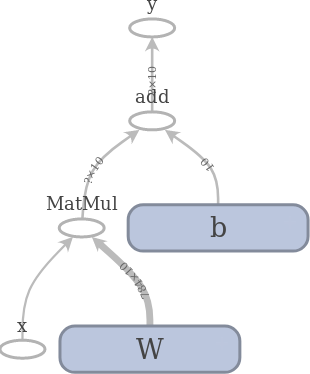
\includegraphics[width=0.45\linewidth]{utils/demo_graph.png}
            \caption{The linear model in graph form.}
        \end{figure}
        \end{column}
    \end{columns}
    \end{block}
    \begin{block}{Operations and Data}
        The expression consists of \operation{operations} that
        are applied to \data{data}:
        \begin{align*}
            y &= \operation{+}\left( \operation{\cdot}(\data{W}, \data{x}), \data{b} \right)
        \end{align*}
        An \operation{operation} is not necessarily a function!
    \end{block}
\end{frame}
    
\begin{frame}
    \frametitle{Why bother?}
    \framesubtitle{Autodifferentiation}
    We don't want to calculate gradients by hand! Use the graph and apply the chain rule automatically.
    %\includegraphics[width=\linewidth]{autodiff}
\end{frame}

\begin{frame}
    \frametitle{Why bother?}
    \framesubtitle{Parallelism}
    \begin{block}{An Ideal World}
    \begin{columns}
    \begin{column}{0.75\linewidth}
        The \data{result} of each \operation{operation} depend only on its input \data{data}. 
        
        Traverse the graph backwards and find all operations whose inputs are \data{data} that is ready.
        These (\operation{a, b, c, d}) can be evaluated in parallel. Whenever an \operation{operation}
        finishes, look if we can start the next one.

        \begin{align*}
            \only<1>{&\operation{f}(\operation{g}(\data{a}, \data{b}), \operation{h}(\data{c}, \operation{d}())}
            \only<2>{&\operation{f}(\data{g}, \operation{h}(\data{c}, \data{d})}
            \only<3>{&\operation{f}(\data{g}, \data{h})}
            \only<4->{&\data{f}}
        \end{align*}
    \end{column}

    \begin{column}{0.25\linewidth}
        \vspace{-2ex}
        \begin{figure}[h]
            \centering
            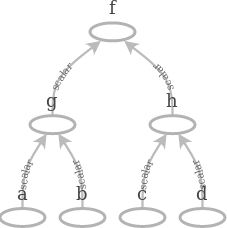
\includegraphics[width=\linewidth]{utils/parallel_graph.png}
            \caption{A parallelizable computation.}
        \end{figure}
    \end{column}
    \end{columns}
    \end{block}

    \begin{block}{The Harsh Reality}<5>
    We want \operation{operations} to be more general than pure functions. Therefore, if one operation depends
    on a side effect of another (but not on data produced by it), we need to add a "fake" (dataless) 
    edge to the graph, called a \emph{\data{control dependency}}.
    \end{block}
\end{frame}

\begin{frame}
    \frametitle{Why bother?}
    \framesubtitle{Efficiency}
    \begin{block}{Acyclic Graphs}
    Calculate only what is needed. Up to now we have considered only trees, but we can use any directed acyclic graph.
    \begin{align}
        x = \operation{f}(\operation{g}(), \operation{h}()), \quad
        y = \operation{s}({\operation{x}(), \operation{h}()}), \quad
        z = \operation{f}(\operation{t}())
    \end{align}
    \end{block}
    \pause
    \begin{block}{Calculation}  
    To calculate $y$ just do the same as before. We will automatically skip useless \operation{operations}
    and compute things only once:
    \only<+>{
    \begin{align}
        x = \operation{f}(\data{g}, \data{h}),\quad
        y = \operation{s}(\operation{x}, \data{h}), \quad
        z = \operation{f}(\operation{t}())
    \end{align}
    }
    \only<+>{
    \begin{align}
        x = \data{f},\quad
        y = \operation{s}(\data{x}, \data{h}), \quad
        z = \operation{f}(\operation{t}())
    \end{align}
    }
    \only<+>{
    \begin{align}
        x = \data{f},\quad
        y = \data{s}, \quad
        z = \operation{f}(\operation{t}())
    \end{align}
    }
    \end{block}
\end{frame}

\begin{frame}
    \frametitle{Why bother?}
    \large{TensorFlow is based on the idea of using a computation graph!}
\end{frame}


\subsection{TensorFlow Basics}
%!TEX root = tfintro.tex

\begin{frame}
    \frametitle{Basic Data Structures}
    \framesubtitle{Overview}
    \begin{block}{Graph}
        The \code{tf.Graph} class manages a computation graph.
    \end{block}
    \begin{block}{Operation}
        The \code{tf.Operation} class represents an \operation{operation}.
    \end{block}
    \begin{block}{Data}
        The \code{tf.Tensor} class represents blobs of \data{data} that are inputs and outputs
        of \operation{operations}.
    \end{block}
    \begin{block}{Executation}
        The \code{tf.Session} class manages the execution of computations and external resources
        that \operation{operations} can interact with.
    \end{block}
\end{frame}

\begin{frame}
    \frametitle{Graphs}
    \framesubtitle{\code{tf.Graph}}
    \begin{block}{Graph objects}
    \code{tf.Graph} objects manage the computational graph. 
    \data{Tensors} and \operation{operations} are identified by a unique name. 
    It also provides \emph{context managers} and some metadata; we'll look at that later.
    \end{block}
    \pause
    \begin{block}{The Default Graph}
        TensorFlow always has a graph as the \emph{default graph} (even if you don't create any graph).
        New \operation{operations} are added to the current default graph.  
    \end{block}
\end{frame}

\begin{frame}
    \frametitle{Operations and Tensors}
    \framesubtitle{\code{tf.Operation}}
    \begin{block}{Operations}
        An \operation{operation} maps \data{inputs} to (possibly multiple) \data{outputs}. 
        It can also have side effects (eg. reading from memory, file system). An operation
        can have \pythonval{attributes} (i.e. parameters that cannot be dynamically set) and be associated
        to a device (e.g. a specific CPU or GPU).
    \end{block}
    \pause
    \begin{block}{Order of Execution}
        An \operation{operation} can be executed once its \data{inputs} (including \data{control dependencies})
        are available. Apart from that \operation{operations} are not further synchronized. An operation is run 
        only once, we assume that the \data{outputs} are fixed once the \data{inputs} are ready. For different 
        executions of the computation, the \operation{operation} may produce different \data{outputs} for
        the same \data{inputs} (e.g. random \operation{ops}).
    \end{block}
\end{frame}


\begin{frame}[fragile]
    \frametitle{Operations and Tensors}
    \framesubtitle{\code{tf.Operation}}
    \begin{block}{Creating Operations}
        \operation{Operations} are usually added to the graph using constructor functions. 
        These functions convert the inputs to \data{tensors} and validate 
        them as far as possible. They do not return the \operation{operation}, but its \data{output},
        which is usually what you need.
        Some examples are
        \begin{lstlisting}
tf.add
tf.multiply
tf.subtract
tf.divide
tf.matmul
tf.constant
        \end{lstlisting}
        Also, the usual math functions like trigonometrics, sqrt, exp etc.
    \end{block}
\end{frame}


\begin{frame}[fragile]
    \frametitle{Operations and Tensors}
    \framesubtitle{Example: \code{tf.constant}}
    \begin{block}{\code{tf.constant}}
        The \code{tf.constant} function does not return an \operation{operation} but a \data{tensor}. 
        Explicitly access its \operation{operation} by the \code{op} attribute. 
        This operation has zero \data{inputs} and one \data{output}. The \pythonval{value} of the constant is fixed at 
        creation time and part of the op definition.
        \begin{lstlisting}
>>> |ta|t = tf.|oconstant|o(|v5|v)
>>> print(|ta|t)
Tensor("Const:0", shape=(), dtype=int32)
>>> print(|oa.op|o)
>>> a.op.graph == tf.get_default_graph()
True
        \end{lstlisting}
    \end{block}
\end{frame}

\begin{frame}[fragile]
    \frametitle{Operations and Tensors}
    \framesubtitle{Example: \code{tf.constant}}
    \begin{block}{The op definition}
        \begin{lstlisting}[morekeywords={name, op, attr, key, value, tensor, dtype, tensor_shape, int_val}]
name: "Const"
op: "Const"
attr {
  key: "dtype"
  value { type: DT_INT32 } 
}
attr {
  key: "value"
  value {
    tensor {
      dtype: DT_INT32
      tensor_shape {}
      int_val: 5
    } 
  }
}
        \end{lstlisting}
    \end{block}
\end{frame}




\begin{frame}
    \frametitle{Operations and Tensors}
    \framesubtitle{\code{tf.Tensor}}
    \begin{block}{Typed Multidimensional Array}
        A \data{\code{tf.Tensor}} \code{T} is a multidimensional array with a \pythonval{fixed data type}. They are the outputs
    of \operation{operations} and their \pythonval{name} contains a number to mark the output index. A \data{tensor} has no 
    \pythonval{value} until the graph is executed!
    \end{block}

    \begin{block}{TensorShape}
        A \data{tensor} has an associated \pythonval{(static) shape} (\code{tf.TensorShape}). 
        It can be partially defined and is available as \pythonval{T.shape}.
        Upon execution, each tensor has a second \data{(dynamic) shape} which always is completely specified.
    \end{block}

    \begin{block}{Overloaded Operators}
        For most python operators (e.g. +, -, *, /, **) the special methods of \code{tf.Tensor} are overloaded.
    \end{block}
\end{frame}

\begin{frame}[fragile]
    \frametitle{Operations and Tensors}
    \framesubtitle{Example: Arithmetic}
    \begin{block}{\code{tf.add}}
        \data{Inputs} to \operation{operations} have to be \data{tensors}, so any python \pythonval{value} you supply
        to \operation{tf.add} is transformed into a \data{tensor} (\operation{tf.constant}). 
        \begin{lstlisting}
>>> |ta|t = tf.|oadd|o(|v3|v, |v5|v)
<tf.Tensor 'Add:0' shape=() dtype=int32>
        \end{lstlisting}
        \pause
        \vspace{2em}
        \centering
        \large
        The result is the \data{tensor}, not the \pythonval{value}!
    \end{block}
    \pause
     \begin{block}{\code{tf.mul}}
        Arithmetic only works if the \data{inputs} have the same type.
        \begin{lstlisting}
>>> |tx|t = tf.|oconstant|o(|v3|v)
>>> |ty|t = tf.|oconstant|o(|v3.5|v)
>>> |tm|t = tf.|omultiply|o(|tx|t, |ty|t)
TypeError
        \end{lstlisting}
    \end{block}
\end{frame}

\begin{frame}
    \frametitle{Data Types}
    \framesubtitle{Basics}
    \begin{block}{Similar to NumPy}
        Tensorflow data types are almost the same as numpy's. 
        A non-exhaustive list:
        \begin{itemize}
            \item signed integers \code{tf.int8}, \ldots, \code{tf.int64}
            \item unsigned integers \code{tf.uint8}, \ldots, \code{tf.uint64}
            \item floating point \code{tf.float32}, \code{tf.float64}
            \item complex numbers \code{tf.complex64}
            \item boolean \code{tf.bool}
            \item byte strings \code{tf.string}
        \end{itemize}
    \end{block}
\end{frame}

\begin{frame}
    \frametitle{Data Types}
    \framesubtitle{Basics}
    \begin{block}{References}
        The data type of a \data{tensor} can also be a reference (e.g. \code{tf.float32\_ref}). 
        In that case the contents of the \data{tensor} can be written to.
    \end{block}
    \begin{block}{Quantized and half-precision}
        For speed (typically during inference) tensorflow also offers half precision (float16) and
        quantized data types.
    \end{block}
    \begin{block}{Default Data Types}
        When converting python \pythonval{values} to \data{tensors} they will be converted to 32 bit types 
        (\code{tf.float32} for floats and \code{tf.int32} for integers). On most GPUs \code{float32} are \emph{much} faster than their 64 bit counterparts. 
    \end{block}
\end{frame}

\begin{frame}[fragile]
    \frametitle{Data Types}
    \framesubtitle{Casting}
    \begin{block}{Strictness}
        TensorFlow is stricter about data types than numpy. 
        You cannot combine \data{tensors} of different data type in arithmetic. 
        \begin{lstlisting}
>>> tf.add(tf.placeholder(tf.int32), tf.placeholder(tf.float32))
Error
        \end{lstlisting}
    \end{block}
    \begin{block}{\code{tf.cast}}
        The \operation{tf.cast} operation creates a new \data{tensor} with a given data type and the "same" value as the \data{input}. 
                \begin{lstlisting}
>>> a = tf.placeholder(tf.int32)
>>> b = tf.placeholder(tf.float32)
>>> tf.add(tf.cast(a, tf.float32), b)
<Tensor ...>
        \end{lstlisting}
    \end{block}
\end{frame}


\begin{frame}
    \frametitle{Sessions}
    \framesubtitle{\code{tf.Session}}
    \begin{block}{Execution}
        Run the graph given some \emph{fetches} (= \data{Tensors} whose \pythonval{value} you want to calculate and retrieve)
        and an optional \emph{feed} dict. The \code{feed\_dict} parameter allows any (feedable) \data{Tensor} to be given a fixed \pythonval{value} so that the graph will not be traversed further.
    \end{block}
    \begin{block}{Resources}
        A session object also manages resources (e.g. allocated memory). 
        These can be temporary (\pythonval{tensors} during a single run) or persistent (the values of \code{tf.Variables}). 
        Therefore it is imperative to close a session after its use to free these resources again. 
    \end{block}
\end{frame}

\begin{frame}[fragile]
    \frametitle{Sessions}
    \framesubtitle{\code{tf.Session}}
    \begin{block}{Fetching Values}
        Replaces \data{tensor} objects with their \pythonval{values} in any nested structure of dicts, lists and tuples.
        \pause
        \begin{lstlisting}
>>> session = tf.Session()
>>> |ta|t = |otf.constant|o(|v5|v)
>>> |tb|t = |otf.constant|o(|v8|v)
>>> session.run([|ta|t, |tb|t])
|v[5, 8]|v
>>> session.run({"a": |ta|t, "b": (|tb|t,)})  
|v{"a": 5, "b": (8,)}|v
        \end{lstlisting}
    \end{block}
\end{frame}

\begin{frame}[fragile]
    \frametitle{Sessions}
    \framesubtitle{\code{tf.Session}}
    \begin{block}{Fetching Operations}
        \operation{Operations} can also be part of the fetch structure. This causes them to be run. 
        Since they have no \pythonval{value} they always return \pythonval{None}.
        \pause
        \begin{lstlisting}
>>> session = tf.Session()
>>> |tx|t = |otf.add|o(|v5|v, |v13|v)
>>> session.run((|tx|t, |ox.op|o))
|v(13, None)|v
        \end{lstlisting}
    \end{block}
\end{frame}

\begin{frame}[fragile]
    \frametitle{Sessions}
    \framesubtitle{\code{tf.Session}}
    \begin{block}{Feeding}
        Feeding a \data{tensor} means that tf assumes that its \pythonval{value} is readily available, so no 
        \operation{operation} has to be invoked to calculate it. 
        \begin{lstlisting}
>>> p = tf.Print(5, [5])
>>> session.run(p)  # prints 5
5
>>> session.run(p, feed_dict={p: 6})  # prints nothing
6
        \end{lstlisting}
    \end{block}
\end{frame}

\begin{frame}[fragile]
    \frametitle{Sessions}
    \framesubtitle{\code{tf.InteractiveSession}}
    \begin{block}{Direct evaluation}
        To get a single \data{tensor} or run a single \operation{operation} it is possible to 
        call \code{run} (for \operation{operations}) or \code{eval} (for \data{tensors}).
        \begin{lstlisting}
>>> a = tf.constant(5)
>>> a.eval(session)
5
        \end{lstlisting}
    \end{block}
    \pause
    \begin{block}{Interactive Session}
        If an \code{InteractiveSession} is used, it will be the \emph{default session} so there is no need to specify it.
        \begin{lstlisting}
>>> session = tf.InteractiveSession()
>>> a = tf.constant(5)
>>> a.eval()
5
        \end{lstlisting}
    \end{block}
\end{frame}

\begin{frame}[fragile]
    \frametitle{Your Turn}
    \begin{block}{Task}
        Transform the following computation into a tensorflow graph. We want to have \code{x} and \code{y} as tensors.
    \begin{lstlisting}
x = 1 + 3
s = 2*x**2 + 5
y = x + np.sqrt(s)
    \end{lstlisting}
    \end{block}
    \pause
    \begin{block}{A Solution}
    Ensure matching data types when passing in \data{tensors}! 
    \pythonval{Python constants} will be automatically cast.
    \begin{lstlisting}
tf.InteractiveSession()
x = tf.add(tf.constant(1.0), tf.constant(3.0))
s = tf.add(tf.multiply(2, tf.pow(x, 2)), 5)
y = tf.add(x, tf.sqrt(s))
y.eval()
    \end{lstlisting}        
    \end{block}
\end{frame}

\begin{frame}[fragile]  % TODO this and the last should be one frame
    \frametitle{Your Turn}
    \begin{block}{Task}
        Transform the following computation into tensorflow graph. We want to have \code{x} and \code{y} as tensors.
    \begin{lstlisting}
x = 1 + 3
s = 2*x**2 + 5
y = x + np.sqrt(s)
    \end{lstlisting}
    \end{block}
    \begin{block}{Using overloaded operators}
    We need at least one \data{tf.Tensor} in the expression to trigger the overloaded operator.
    \begin{lstlisting}
tf.InteractiveSession()
x = tf.constant(1.0) + 3
s = 2*x**2 + 5
y = x + tf.sqrt(s)
y.eval()
    \end{lstlisting}        
    \end{block}
\end{frame}


\begin{frame}[fragile]
    \frametitle{Recap}
    Building a Graph is like \emph{defining} a python function, where the \operation{ops} are the instructions 
    and \data{tensors} are \emph{immutable} local variables. Running the graph in a session is like executing 
    the function in a python interpreter.
    \pause
    \begin{columns}
    \begin{column}{0.5\textwidth}
    \begin{lstlisting}
a = tf.constant(5)
b = tf.constant(10)
x = tf.add(a, b)
    \end{lstlisting}
    \end{column}
    \begin{column}{0.5\textwidth}
    \begin{lstlisting}
def calculate_x():
    a = 5
    b = 10
    x = a + b
    return x
    \end{lstlisting}
    \end{column}
    \end{columns}
    \pause
    At this point, no calculations have been performed yet. For that we need to actually call the function.
    \begin{columns}
    \begin{column}{0.5\textwidth}
    \begin{lstlisting}
session.run(x)
    \end{lstlisting}
    \end{column}
    \begin{column}{0.5\textwidth}
    \begin{lstlisting}
calculate_x()
    \end{lstlisting}
    \end{column}
    \end{columns}
    \pause
    What is missing still is the equivalent of function \emph{arguments} and \emph{global variables}.
\end{frame}


\subsection{Placeholders and Variables}
%!TEX root = tfintro.tex

\begin{frame}[fragile]
    \frametitle{Placeholders}
    \framesubtitle{Arguments for the Graph}
    A placeholder is an \operation{operation} that cannot be evaluated. 
    If its \data{value} is needed it has to be fed.
     \begin{lstlisting}
>>> p = tf.placeholder(tf.float32)
>>> a = tf.add(p, 1.0)
>>> a.eval()
Error
>>> a.eval(feed_dict={p: 2.0})
3.0
     \end{lstlisting}
\end{frame}

\begin{frame}
    \frametitle{Shapes}
    \framesubtitle{\code{tf.TensorShape}}
    \begin{block}{Partial Shapes}
        The most unspecific shape possible is \pythonval{tf.TensorShape(None)} which can be any arbitrary shape.
        We can also just specify the rank \pythonval{tf.TensorShape([None, None])} or single dimensions
        \pythonval{tf.TensorShape([None, 10])}.
    \end{block}
    \begin{block}{Guarantees on Dynamic Shapes}
        A static shape is just a guarantee we specify for the dynamical shape. Example: If \data{y} is a tensor 
        of static shape \pythonval{[None, 10]} and gets assigned data of shape \data{[5, 10]} everything is fine, but if we try to assign \data{[5, 15]} an error is raised.
    \end{block}
    \begin{block}{Automatic Shape Inference}
        Most python functions that create \operation{operations} also perform automatic shape inference.
        (\operation{add}(a.shape=\pythonval{[None, 10]}, b.shape=\pythonval{[5, None]})).shape == [5, 10]).
    \end{block}
\end{frame}

\begin{frame}[fragile]
    \frametitle{Shapes}
    \framesubtitle{Broadcasting}
    \begin{block}{Rules as in numpy}  % TODO I think so, look that up 
        Broadcasting works similarly to numpy and usually "does the right thing". 
        Singleton dimensions (dimensions with size 1) will be expaned to match the dimension of the other \data{tensor} and missing dimensions are of size 1. 
    \end{block}
    \pause
    \begin{block}{Examples}
    \begin{lstlisting}
>>> a = tf.constant(1.0)
>>> b = tf.constant([1.0, 2.0, 3.0])
>>> (a+b).eval()
[2.0, 3.0, 4.0]
    \end{lstlisting}
    \end{block}
\end{frame}

\begin{frame}
    \frametitle{Variables}
    \framesubtitle{Storing values across run calls.}
    \begin{block}{Not a single graph object.}
        A \emph{Variable} is modeled by the \code{tf.Variable} class and not a single \operation{operation} or \data{tensor}, 
        but an interface for interaction with a region of memory. It can construct \operation{operations} for
        reading and writing data and an for assigning the \data{initial value}.
    \end{block}
    \begin{block}{Creating a Variable}
        A variable can be created using \code{tf.Variable} which needs at least an \data{initial value}.
        It can also be named and get its \pythonval{data type} specified. 
    \end{block}
\end{frame}

\begin{frame}[fragile]
    \frametitle{Variables}
    \framesubtitle{Storing values across run calls.}
    \begin{block}{Assignments}
        To assign a a new value the \operation{assign} operation can be used. 
        \begin{lstlisting}
tf.assign(|tref|t, |tvalue|t, |vvalidate_shape|v=None, |vuse_locking|v=None, |vname|v=None)
        \end{lstlisting}
        To change the shape of the variable, set \code{validate\_shape} to \code{False}. Assign is also available as a method of the 
        \code{Variable} class.
    \end{block}
    \begin{block}{Initialization}
        A variable cannot be read from until it has been assigned a value. For the first time, this is done 
        by its \operation{initialization op}. Alternatively, the initial value can be read from a save file and
        be assigned to the Variable. To initialize all variables at once, run the \operation{operation} created 
        by \code{tf.global\_variables\_initializer()}.
    \end{block}
\end{frame}

% Variable initialization, initialized_value
% assign, assign_add, etc
% full example

%%% NEURAL NETWORKS %%%
\section{Training Neural Networks}
\subsection{Neural Networks and Training}
%!TEX root = tfintro.tex

\begin{frame}[fragile]
    \frametitle{Some More Operations}
    \framesubtitle{Constant tensors}
    \operation{Operations} with constant \data{output}: 
    \begin{lstlisting}  
tf.zeros(|tshape|t, dtype=tf.float32, name=None)
tf.ones(|tshape|t, dtype=tf.float32, name=None)
tf.fill(|tdims|t, |tvalue|t, name=None)
tf.constant(|vvalue|v, dtype=None, shape=None, name='Const', 
            verify_shape=False)
    \end{lstlisting}
    \pause
    And for your convenience
    \begin{lstlisting}  
tf.zeros_like(|ttensor|t, dtype=None, name=None, optimize=True)
tf.ones_like(|ttensor|t, dtype=None, name=None, optimize=True)
    \end{lstlisting}
    \pause
    Why not just \operation{tf.constant}?
    \pause
    Because then all those zeros/ones need to be saved inside an \pythonval{attribute} of the \operation{op},
    whereas \operation{tf.zeros} can create them on the fly. Also readability.
\end{frame}

\begin{frame}[fragile]
    \frametitle{Some More Operations}
    \framesubtitle{Reductions}
    Performing operations over all elements of one or more dimensions. They all share the same function signature.
    For numerical data
    \begin{lstlisting}  
tf.reduce_sum(|tinput_tensor|t, |vaxis=None|v, keep_dims=False, name=None)
tf.reduce_prod, tf.reduce_max, tf.reduce_min, 
tf.reduce_logsumexp
    \end{lstlisting}
    and for booleans / strings
    \begin{lstlisting}  
tf.reduce_any, tf.reduce_all
tf.reduce_join
    \end{lstlisting}
\end{frame}

\begin{frame}[fragile]
    \frametitle{Linear Model}
    \framesubtitle{Forward pass}
    We now have everything to build the forward pass of a simple linear model.
    \begin{lstlisting}  
W = tf.Variable(np.random((10, 784)))
b = tf.Variable(np.random(10))
x = tf.placeholder(tf.float32, (None, 784))
l = tf.matmul(W, x) + b
    \end{lstlisting}
    \pause
    Now we need to convert this into a probability distribution over classes, 
    and a \emph{loss} function as optimization objective. Typical in classification tasks:
    \emph{softmax} nonlinearity and \emph{cross-entropy} loss.
\end{frame}

\begin{frame}
    \frametitle{Linear Model}
    \framesubtitle{Classification}
    Classification task: Exactly one of $k$ classes is true.
    \begin{block}{Softmax}
        \[
            \mathrm{softmax}(x)_i = \frac{\exp(x_i)}{\sum_{j=1}^k \exp(x_j)}.
        \]
    \end{block}
    \begin{block}{Cross-Entropy}
    Let $p(i)$ be the true probability of class $i$ and $q(i)$ be the predicted probability.
    The cross-entropy between the two distributions is
    \[
        X(p, q) = \sum_{i=1}^{k} p(i) \log q(i).
    \]
    "How good can we compress data distributed $\sim p$ if we assume it is distributed $\sim q$"
    \end{block}
\end{frame}

\begin{frame}[fragile]
    \frametitle{Linear Model}
    \framesubtitle{Loss Function}
    \begin{lstlisting}
y = tf.placeholder(tf.float32, (None, 10))
p = tf.nn.softmax(l)
loss = tf.nn.softmax_cross_entropy_with_logits(labels=y, logits=l)
    \end{lstlisting}
    \begin{block}{Some Notes}
        \begin{itemize}
            \item The function takes in logits instead of probabilities for numerical stability.
            \item Labels need not be one-hot vectors, but can be arbitrary probablity distributions over classes.
        \end{itemize}
    \end{block}
\end{frame}

\begin{frame}
    \frametitle{Stochastic Gradient Descent}
    \framesubtitle{Optimizing Differentiable Functions}
    \begin{block}{Gradient Descent}
        Function $f$ of input dataset $X=(x_1, \ldots, x_n)$ and \emph{weights} $\theta$, loss $L$ and target values $Y=(y_1, \ldots, y_n)$, learning rate $\alpha$
        \begin{align}
            \theta \leftarrow \theta + \alpha \nabla_\theta L(f(X; \theta), Y)
        \end{align}
    \end{block}
    \begin{block}{Estimating from Minibatches}
        \begin{align*}
            \nabla_\theta L(f(X; \theta), Y) = \sum_{i=1}^{n} \nabla_\theta L(f(x_i; \theta), y_i) = \frac{n}{k} \cdot \mathbb{E}\left[\sum_{i=1}^{k} \nabla_\theta L(f(x_{j_i}; \theta), y_{j_i})\right]
        \end{align*}
        For uniformly sampled $j_i$ we can use the rhs. as an unbiased estimator for the true gradient. 
        $\Rightarrow$ \emph{Stochastic Gradient Descent}.
    \end{block}
\end{frame}

\begin{frame}[fragile]
    \frametitle{Optimizers}
    \framesubtitle{This Could be Your Slide about Backpropagation \ldots}
    \begin{block}{Autodifferentiation is Your Friend}
        As long as each \operation{operation} used in the mapping from \data{input} to \data{loss} tensor 
        is \emph{differentiable} we need not worry about calculating the gradient of the chained \operation{operation}.
    \end{block}

    \begin{block}{Minimizing the Loss}
        \begin{lstlisting}
train_step = tf.train.GradientDescentOptimizer(0.1).minimize(loss)
        \end{lstlisting}
        The result is an \operation{operation} that performs a single gradient descent step when run. 
        This means calculating the gradients and updating the trainable variables.
    \end{block}
\end{frame}

\begin{frame}[fragile]
    \frametitle{The Full Network}
    \begin{block}{Network Code}
        \begin{lstlisting}
x = tf.placeholder(tf.float32, (None, 784))
y = tf.placeholder(tf.float32, (None, 10))
W = tf.Variable(np.random((10, 784)))
b = tf.Variable(np.random(10))
l = tf.matmul(W, x) + b
p = tf.nn.softmax(l)
loss = tf.nn.softmax_cross_entropy_with_logits(labels=y, logits=l)
train_step = tf.train.GradientDescentOptimizer(0.1).minimize(loss)
        \end{lstlisting}        
    \end{block}
\begin{block}{Getting Data}
        \begin{lstlisting}
import tensorflow.contrib.learn as tflearn
mnist = tflearn.datasets.load_dataset("mnist")
images = mnist.train.images
labels = mnist.train.labels
        \end{lstlisting}        
    \end{block}
\end{frame}

\begin{frame}[fragile]
    \frametitle{Basic Linear Model}
    \centering Notebook (01 Linear Model.ipynb)
\end{frame}


\subsection{Summaries and Tensorboard}
%!TEX root = tfintro.tex

\begin{frame}
	\frametitle{Summaries}
	\framesubtitle{Gather Monitoring Data inside the Graph}
	Add graph \operation{operations} responsible for logging (\emph{summaries}).
	\begin{block}{Motivation}
		\begin{itemize}
			\item On-line monitoring of progress (e.g. loss, accuracy) and network internals (e.g. weight norms, regularization losses)
			\item Feed-dict does not scale well to many summaries.
			\item High level debugging. See that input images are correctly preprocessed, gradient norms remain reasonable etc. 
		\end{itemize}
	\end{block}
	\begin{block}{Summary Operations}
		Take in a \data{Tensor} and produce a string \data{summary} (which is a serialized protobuf object). These can be collected and written to a summary file. 
	\end{block}
\end{frame}

\begin{frame}
	\frametitle{Summaries}
	\framesubtitle{Gather Monitoring Data inside the Graph}
	\begin{block}{Summary Types}
	The following summaries are available in the \code{tf.summary} module.
	\begin{description}
		\item[scalar] A single real value, e.g. the loss.
		\item[histogram] Histogram of the values of a \data{Tensor}, e.g. to visualize distributions of activations.
		\item[image] An image [$\mathrm{Batch}\times\mathrm{Height}\times\mathrm{Width}\times\mathrm{Channels}$] tensor. 
		\item[audio] Audio data in format [$\mathrm{Batch}\times\mathrm{Frames}\times\mathrm{Channels}$] or [$\mathrm{Batch}\times\mathrm{Frames}$] in range $[-1.0, 1.0]$.
		\item[text] A string tensor representing textual data.
	\end{description}
	Each \operation{summary} takes at least two arguments: A \pythonval{name} (or tag) for the operation, and
	the \data{tensor} to summarize.  
	\end{block}
\end{frame}

\begin{frame}[fragile]
	\frametitle{Summaries}
	\framesubtitle{Gather Monitoring Data inside the Graph}
	\begin{block}{Merging Summaries}
		Since summaries are \operation{operations}, we need to explictly pass them as fetches to generate summary values.
		To make this more usable, multiple \data{summaries} can be \operation{merged} into a single \data{summary}. 
		This can be done for an explicit list of summaries (\code{tf.summary.merge}) or for all summaries in the graph
		(\code{tf.summary.merge\_all}).
	\end{block}
	\begin{block}{Example}
		\begin{lstlisting}
a = tf.summary.scalar("loss", loss)
b = tf.summary.scalar("accuracy", accuracy)
s = tf.summary.merge_all()   # = tf.summary.merge([a, b])
		\end{lstlisting}
		To generate the summaries during training:
		\begin{lstlisting}
_, summary = session.run([train_step, s], feed_dict=feed_dict)
		\end{lstlisting}
		Gets both "loss" and "accuracy" summaries.
	\end{block}
\end{frame}

\begin{frame}[fragile]
	\frametitle{Summary Writer}
	\framesubtitle{Saving Summaries}
	\begin{block}{FileWriter}
		A \code{tf.summary.FileWriter} is responsible for writing log \emph{events} to a file. 
		Events can be summaries, graphs, session logs, run metadata etc. 
		\begin{lstlisting}
tf.summary.FileWriter(logdir, graph, max_queue, flush_secs, filename_suffix)
		\end{lstlisting}
		Creates a new summary file with a unique name inside \texttt{logdir} and
		writes a graph event to it if \code{graph} is supplied.
	\end{block}
	\begin{block}{Directories Group Runs}
	By convention \textbf{all} event files within a single directory are assumed to be from the same 
	\emph{run}. These containing events will be grouped together.
	% Correct and wrong example images here.
	\end{block}
\end{frame}

\begin{frame}[fragile]
	\frametitle{Summary Writer}
	\framesubtitle{Saving Summaries}
	\begin{block}{Adding Events to Summary Files}
	To add a summary one needs the (serialized) Protocol Buffer and an associated \emph{global step}. 
	\begin{lstlisting}
summary = session.run(|tsummaries|t)
writer.add_summary(|vsummary|v, |vglobal_step|v)
	\end{lstlisting}
	While the step is typically gathered from a \data{global\_step} variable, the summary writer accepts 
	any \pythonval{python integer}. The step is used to form a time axis for your log data.
	\end{block}
	\begin{block}{Writes Are Asynchronous}
	To prevent training slowdowns by summary writes, the \code{FileWriter} writes only asynchronously to 
	the summary file. This can be controlled with the \code{max\_queue} and \code{flush\_secs} parameters.
	\end{block}
\end{frame}

\begin{frame}[fragile]
    \frametitle{Some More Operations}
    \framesubtitle{Comparisons}
    \begin{block}{Comparison Operations}
    Compare tensors element-wise
    \begin{lstlisting}  
tf.equal(|tx|t, |ty|t, |vname|v=None)
    \end{lstlisting}
    and analogly
    \begin{lstlisting}  
tf.less, tf.less_equal, tf.greater, tf.greater_equal
    \end{lstlisting}
    \pause
    Booleans to numbers
    \begin{lstlisting}
tf.cast(|tbool_tensor|t, |vdata_type|v)
    \end{lstlisting}
    converts every \code{True} to $1.0$ and every \code{False} to $0.0$.    	
    \end{block}
	\begin{block}{Calculating Accuracy}
	\begin{lstlisting}
is_correct = tf.equal(tf.argmax(|tlogits|t, axis=1), |ty|t)
accuracy = tf.reduce_mean(tf.cast(is_correct, |vtf.float64|v))
    \end{lstlisting}
	\end{block}
\end{frame}

\begin{frame}[fragile]
	\frametitle{Linear Model with Summaries}
	\centering Notebook (02 Summaries.ipynb)
\end{frame}

\begin{frame}[fragile]
	\frametitle{Tensorboard}
	\centering
	Tensorboard Demo
\end{frame}
{}

\subsection{Checkpointing}
%!TEX root = tfintro.tex

\begin{frame}[fragile]
    \frametitle{tf.train.Saver}
    \framesubtitle{Writing Variables to Files}
    The Saver class is responsible for building \operation{operations} that save and restore Variables to/from a checkpoint file.
    \begin{lstlisting}
tf.train.Saver(|mvar_list|m=None, reshape=False, max_to_keep=5, 
keep_checkpoint_every_n_hours=10000.0, 
name=None, restore_sequentially=False, saver_def=None, 
builder=None, defer_build=False, allow_empty=False, 
save_relative_paths=False, filename=None)
    \end{lstlisting}
    \begin{description}
        \item[var\_list] List (or dictionary) of Variables to save. If \code{None} is submitted all \emph{global variables} are saved.
        \item[max\_to\_keep] How many checkpoint files to keep before starting to delete older ones.
    \end{description}
    Creating a Saver does not yet save anything!
\end{frame}

\begin{frame}[fragile]
    \frametitle{tf.train.Saver}
    \framesubtitle{Writing Variables to Files}
    \begin{block}{Saving to a Checkpoint}
        Create a Saver object \textbf{after} the model has been build. Then
        \begin{lstlisting}
saver.save(session, |vsave_path|v, |tglobal_step|t=None, |vlatest_filename|v=None)
        \end{lstlisting}
        This saves the model to  \code{save\_path}, and if \code{global\_step} is supplied also
        registers the new checkpoint in the \emph{latest checkpoints file} (named \code{"checkpoint"} or 
        \code{latest\_filename}).
    \end{block}

    \begin{block}{Step Counting}
        Save step count inside a tf.Variable to have consistent counts across checkpoints. Either manually or using 
        \begin{lstlisting}
global_step = tf.Variable(0, dtype=tf.int64, trainable=False)
global_step = tf.train.create_global_step()
        \end{lstlisting}
        Automatically increment the global step for each optimization step.
        \begin{lstlisting}
train_step = optimizer.minimize(loss, global_step=global_step)
        \end{lstlisting}
    \end{block}
\end{frame}

\begin{frame}[fragile]
    \frametitle{tf.train.Saver}
    \framesubtitle{Restoring}
    \begin{block}{Loading a Checkpoint}
    To load the values into an \emph{already existing} model do
\begin{lstlisting}
saver.restore(session, |vsave_path|v)
\end{lstlisting}
To also restore the graph call create your saver as
\begin{lstlisting}
new_saver = tf.train.import_meta_graph(|vmeta_graph_file_name|v)
\end{lstlisting}
    \end{block}

    \begin{block}{Finding the Correct Checkpoint File}
        To restore you need the complete checkpoint file name, including the step suffix.
        This can be found using the \code{latest\_checkpoint} function:
    \begin{lstlisting}
checkpoint = tf.train.latest_checkpoint(|vcheckpoint_dir|v ,|vlatest_filename|v=None)
saver.restore(session, checkpoint)
    \end{lstlisting}
    \end{block}
\end{frame}

\begin{frame}[fragile]
    \frametitle{Linear Model with Checkpoints}
    \centering Notebook (03 Checkpoints.ipynb)
\end{frame}

\subsection{Structuring a Model}
%!TEX root = tfintro.tex

\begin{frame}[fragile]
    \frametitle{Useful Python Features}
    \begin{block}{Context Managers}
        Allows do some code in a certain context by executing an \code{\_\_enter\_\_} function when the context starts
        and an \code{\_\_exit\_\_} function when the context ends. For example:
\begin{lstlisting}
with open("filename") as file:
    # do sth with the file
# here, the file will be close again
\end{lstlisting}
    This is used extensively by tensorflow for default sessions, default graphs, devices, scoping etc.
    \end{block}
    \begin{block}{Named Tuples}
        Makes a helper type that behaves like a tuple, but can be indexed with named keys.
\begin{lstlisting}
NamedTuple = namedtuple("NamedTuple", ("a", "b"))
data = NamedTuple(a=5, b="test")
\end{lstlisting}        
    \end{block}
\end{frame}

\begin{frame}[fragile]
    \frametitle{Default Session and Default Graph}
    \framesubtitle{}
    \begin{columns}
        \begin{column}{0.4\linewidth}
        Instead of 
        \begin{lstlisting}
# build your model here
session = tf.Session()
# your main loop here
session.close()
    \end{lstlisting}
    \begin{block}{Problems}
    \begin{itemize}
        \item Risks forgetting to close session. 
                Leaks in case of exception.
        \item Pollutes global default graph. 
    \end{itemize}
    \end{block}
        \end{column}
        \begin{column}{0.5\linewidth}
        Do
    \begin{lstlisting}
graph = tf.Graph()
with graph.as_default():
    # build your model here
with tf.Session(graph=graph) as session:
    # Your main loop here
    \end{lstlisting}
        \begin{block}{Advantages}
    \begin{itemize}
        \item Guaranteed cleanup.
        \item Can easily create multiple graphs and runs in a single program without interference.
    \end{itemize}
    \end{block}
        \end{column}
    \end{columns}
\end{frame}

\begin{frame}[fragile]
    \frametitle{Model Function}
    \framesubtitle{Separating Model Definition and Training Routine}
        Instead of building the model inside the default graph, put the model into its own function.
        Keep the model inputs as arguments.
    \begin{lstlisting}
Model = namedtuple("Model", ("loss", "train_step"))

def model_fn(x, y):
    W = tf.Variable(np.random((10, 784)))
    b = tf.Variable(np.random(10))
    l = tf.matmul(W, x) + b
    labels = tf.one_hot(y, depth=10)
    loss = tf.nn.softmax_cross_entropy_with_logits(labels=labels, logits=l)
    loss = tf.reduce_mean(loss)
    train_step = tf.train.GradientDescentOptimizer(0.1).minimize(loss)
    return Model(loss=loss, train_step=train_step)
    \end{lstlisting}
\end{frame}


\begin{frame}[fragile]
    \frametitle{Model Function}
    \framesubtitle{Separating Model Definition and Training Routine}
    Use as follows:
    \begin{lstlisting}
graph = tf.Graph()
with graph.as_default():
    x = tf.placeholder(tf.float32, (None, 784), name="x")
    y = tf.placeholder(tf.int64, (None), name="y")  
    loss, train_step = model_fn(x, y)
    init_op = tf.global_variables_initializer()

with tf.Session(graph=graph) as session:
    init_op.run()
    # Your main loop here
    \end{lstlisting}
\end{frame}

\begin{frame}[fragile]
    \frametitle{Scoping}
    \framesubtitle{Structure in Operation Names}
    \begin{block}{Name Scopes}
        Every operation created within a name scope will have its name 
        prefixed by that scope name.
            \begin{lstlisting}
with tf.name_scope("prefix"):
    a = tf.add(5, 4)
print(a.name)  #  "prefix/Add:0"
    \end{lstlisting}
    \end{block}

    \begin{block}{Nesting}
        Name scopes stack.
    \begin{lstlisting}
with tf.name_scope("prefix"):
    with tf.name_scope("inner"):
        a = tf.add(5, 4)
print(a.name)  #  "prefix/inner/Add:0"
    \end{lstlisting}
    \end{block}
\end{frame}

\begin{frame}[fragile]
    \frametitle{Scoping}
    \framesubtitle{Structure in Operation Names}
    \begin{block}{Re-Opening Name Scopes}
        Using the same name scope again will create a new, unique prefix 
        \begin{lstlisting}
with tf.name_scope("prefix"):
    a = tf.add(5, 4)
with tf.name_scope("prefix"):
    a = tf.add(5, 4)
print(a.name)  #  "prefix_1/Add:0"
        \end{lstlisting}
        But you can remember a scope and reuse it as an absolute scope.
        \begin{lstlisting}
with tf.name_scope("prefix") as prefix_scope:
    pass
with tf.name_scope("other"):
    with tf.name_scope(prefix_scope):
        a = tf.add(5, 4)
print(a.name)  #  "prefix/Add:0"
        \end{lstlisting}
    \end{block}
\end{frame}

\begin{frame}[fragile]
    \frametitle{Scoping}
    \framesubtitle{Variable Reuse}
    \begin{block}{Weight Sharing}
        In some models we want to use the same weights in different parts of the computation (e.g. in a GAN).
        This can be achieved using \emph{variable scopes}.
    \end{block}
    \begin{block}{Variable Scope}
        A variable scope sets the name scope in which variables are created or looked up. Use in conjunction with
        \code{tf.get\_variable} which either gets an existing variable or creates a new variable. Opening a variable 
        scope of the same name again will open the \emph{exact same scope}
\begin{lstlisting}
with tf.variable_scope("S"):
    tf.get_variable("a", shape=()).name  # S/a:0
with tf.variable_scope("S"):
    tf.get_variable("b", shape=()).name  # S/b:0
        \end{lstlisting}
    \end{block}
\end{frame}

\begin{frame}[fragile]
    \frametitle{Scoping}
    \framesubtitle{Variable Reuse}
    \begin{block}{Reusing a Scope}
        Inside a variable scope you can either create new variables \textbf{or} reuse existing ones, never both:
\begin{lstlisting}
with tf.variable_scope("S"):
    tf.get_variable("a", shape=()).name  # S/a:0
with tf.variable_scope("S"):
    tf.get_variable("a", shape=()).name  # ERROR
with tf.variable_scope("S", reuse=True):
    tf.get_variable("a").name  # S/a:0
\end{lstlisting}
Entering a non-reusing scope as subscope inside a reusing one is not possible, and neither is the reverse:
    \begin{lstlisting}
with tf.variable_scope("S", reuse=True):
    with tf.variable_scope("T", reuse=False)
        pass  # ERROR
\end{lstlisting}
    \end{block}
\end{frame}

\begin{frame}[fragile]
    \frametitle{Scoping}
    \framesubtitle{Variable Reuse}
    \begin{block}{Variable Scopes and Name Scopes}
        Entering a Variable Scope automatically enters a name scope of the same name.
\begin{lstlisting}
with tf.name_scope("other") as other_scope:
    pass
with tf.variable_scope("S"):
    tf.get_variable("a", shape=())
with tf.variable_scope("S", reuse=True):
    tf.add(5, 4)  # S_1/Add:0
    with tf.name_scope(other_scope):
        a = tf.get_variable("a", shape=())  # S/a:0
        tf.add(a, 4)  # other/Add:0
\end{lstlisting}
    \end{block}
\end{frame}

\begin{frame}[fragile]
    \frametitle{get\_variable}
    \framesubtitle{A Imporved Interface to Variables}
    \code{get\_variable} acts as a Variable constructor that respects the current variable scope.
\begin{lstlisting}
tf.get_variable(name, shape=None, dtype=None, initializer=None, 
                regularizer=None, trainable=True, |gcollections=None, 
                caching_device=None, partitioner=None|g, 
                validate_shape=True, |guse_resource=None, 
                custom_getter=None|g, constraint=None)
\end{lstlisting}
    Instead of an initial value, an \code{initializer} has to be passed. 
    This is a \buildfun{function} that takes in the desired shape and data type
    and \operation{produces} the \data{initial value}. The \buildfun{regularizer}
    is a function that takes the variables \data{value} and outputs a 
    \emph{regularization} \data{loss}, and \buildfun{constraint} maps the 
    variables \data{value} to a constrained \data{value}.
\end{frame}

\begin{frame}
    \frametitle{Graph Building Functions}
    \framesubtitle{Passing Around Recipies for Subgraphs}
    \begin{block}{Building Functions}
    Passing around \buildfun{building functions} instead of pre-built \data{tensors}
    allows to build computations in the correct context.
    \begin{description}
        \item[initializer] The initial value is calculated in the Variable's name scope.
        \item[constraint] The constraint should be applied after an update to the variable, but 
        this has not happened yet at construction time.
    \end{description}        
    \end{block}

    \begin{block}{Another Level of Indirection}
        \[\mathrm{building ~ function} \stackrel{\mathrm{build}}{\longrightarrow} \mathrm{computation ~ graph} \stackrel{\mathrm{run}}{\longrightarrow} \mathrm{values}
     \]
    \end{block}
\end{frame}

\begin{frame}[fragile]
    \frametitle{Initializer}
    \framesubtitle{Building Functions for Initial Values}
    The following initializers are available in tensorflow:
\begin{lstlisting}
zeros(dtype=tf.float32)
ones(dtype=tf.float32)
constant(value=0, dtype=tf.float32, verify_shape=False, dtype=tf.float32)
random_uniform(minval=0, maxval=None, seed=None, dtype=tf.float32)
random_normal(mean=0.0, stddev=1.0, seed=None, dtype=tf.float32)
truncated_normal(mean=0.0, stddev=1.0, seed=None, dtype=tf.float32)
variance_scaling(scale=1.0, mode="fan_in", distribution="normal", 
                 seed=None, dtype=tf.float32)
orthogonal(gain=1.0, seed=None, dtype=tf.float32)
identity(gain=1.0, dtype=tf.float32)
\end{lstlisting}
The functions are available as \code{tf.*\_initializer} or \code{tf.initializers.*}
\end{frame}

\begin{frame}
    \frametitle{Random Operations}
    \framesubtitle{Deterministic Pseudo-Random Numbers}
    To get deterministic pseudo-random numbers, a (graph level) random seed has to be set by
    \code{tf.set\_random\_seed}. In addition, each random operation has its own seed. The randomization
    is then as follows
    \begin{description}
        \item[both not set] A random seed is generated for each run and operation.
        \item[graph seed is set] Operation seeds are picked deterministically from the graph seed.
        \item[operation seed set] Use a default graph seed together with the operation seed.
        \item[both set] Combine graph and operation seed. 
    \end{description}
\end{frame}

\begin{frame}[fragile]
    \frametitle{Random Operations}
    \framesubtitle{List of Ops}
    \begin{block}{Drawing from a Distribution}
    All operations below also do have a \code{seed} and a \code{name} argument.
    \begin{lstlisting}
tf.random_normal(shape, mean=0.0, stddev=1.0, dtype=tf.float32)
tf.truncated_normal(shape, mean=0.0, stddev=1.0, dtype=tf.float32)
tf.random_uniform(shape, minval=0, maxval=None, dtype=tf.float32)
tf.random_gamma(shape, alpha, beta=None, dtype=tf.float32)
tf.multinomial(logits, num_samples)
\end{lstlisting}       
    \end{block}

    \begin{block}{Modify Existing Values}
        \begin{lstlisting}
tf.random_shuffle(value, seed=None, name=None)
tf.random_crop(value, size, seed=None, name=None)
\end{lstlisting}
    \end{block}
\end{frame}

\begin{frame}[fragile]
    \frametitle{Graph Collections}
    \framesubtitle{Categorizing Ops and Tensors}
    \begin{block}{}
    Functions like \code{merge\_all\_summaries}, \code{global\_variables\_initializer}, etc need to find the graph elements that they should operate on.
    This is facilitated by graph collections.
    \end{block}
    \begin{block}{Graph Collection}
        A graph collection is a list of graph elements that is registered under a certain name in the graph.
        \begin{lstlisting}
tf.get_collection(key, scope=None)
tf.add_to_collection(name, value)
        \end{lstlisting}
        These collections then allow to categorize tensors according to their purpose.
    \end{block}
\end{frame}

\begin{frame}[fragile]
    \frametitle{Graph Collections}
    \framesubtitle{Standard Collections}
    By default tensorflow uses the among others following collection keys (all defined in \code{tf.GraphKeys})
    \begin{description}
        \item[GLOBAL\_VARIABLES] All model weights, global step etc.
        \item[TRAINABLE\_VARIABLES] Variables that will be updated by the optimizer.
        \item[SUMMARIES] All summaries.
        \item[REGULARIZATION\_LOSSES] All regularization losses.
    \end{description}
    \vspace{2em}
    More keys are only used by subsystems
    \begin{description}
        \item[GLOBAL\_STEP] The global step variable when used with \code{tf.train}.
        \item[LOSSES] Losses built with \code{tf.losses}
        \item[WEIGHTS, BIASES] Kernels and biases of \code{tf.layers}
    \end{description}
\end{frame}

\begin{frame}[fragile]
    \frametitle{Linear Model}
    \centering Notebook (04 Structure.ipynb)
\end{frame}

\begin{frame}
    \centering
    Notebook (05 Higher Level.ipynb)
\end{frame}

% images of the graphs?
% putting things together

%%% Higher Level Interface %%%
\section{Higher Level Interface}
\subsection{Layers}
%!TEX root = tfintro.tex

\begin{frame}
    \frametitle{Layers Interface}
    \framesubtitle{Quickly Building Sequential Models}
    The functions in \code{tf.layers} take an input value and build a complete neural network \emph{layer} that transforms the value.
    This includes inferring the shapes of the invoved tensors and creating or reusing variables. 
    There are layers for
    \begin{itemize}
        \item Flattening
        \item Dense (fully connected) multiplication
        \item Convolution
        \item Max Pooling
        \item Dropout
        \item Batch Normalization 
    \end{itemize}
    \pause
    If your favourite layer is not listed here, the necessary primitives might still be in \code{tf.nn}, or it might be in \code{tf.contrib}.
\end{frame}

\begin{frame}[fragile]
    \frametitle{Dense Layer}
    \framesubtitle{Argument Overview}
    Most layer functions take a vast amount of arguments. There are three per variable for \emph{initializer}, \emph{regularizer} and \emph{constraint}.
    \begin{onlyenv}<1>
    \begin{lstlisting}
tf.layers.dense(
    |tinputs|t,
    |vunits|v,
    |factivation|f=None,
    |vuse_bias|v=True,
    |fkernel_initializer|f=None,
    |fbias_initializer|f=tf.zeros_initializer(),
    |fkernel_regularizer|f=None,
    |fbias_regularizer|f=None,
    |factivity_regularizer|f=None,
    |fkernel_constraint|f=None,
    |fbias_constraint|f=None,
    |vtrainable|v=True,
    |vname|v=None,
    |vreuse|v=None
)
    \end{lstlisting}
    \end{onlyenv}
    \begin{onlyenv}<2>
    \begin{lstlisting}
tf.layers.dense(
    |tinputs|t,
    |vunits|v,
    |factivation|f=None,
    |vuse_bias|v=True,
    |factivity_regularizer|f=None,
    |vtrainable|v=True,
    |vname|v=None,
    |vreuse|v=None
)
    \end{lstlisting}
    \code{name}, \code{reuse} and \code{trainable} are also passed for the variables and determine variable scope, reuse and trainability. \code{activity\_regularizer} adds 
    a regularization loss depending on the layers output. 
    \end{onlyenv}
\end{frame}

\begin{frame}[fragile]
    \frametitle{Dense Layer}
    The main interface of the layer is
    \begin{lstlisting}
tf.layers.dense(|tinputs|t, |vunits|v, |factivation|f=None, |vuse_bias|v=True)
    \end{lstlisting}
    \begin{block}{Arguments}
        \begin{description}
        \item[inputs] Input tensor $x$ of shape \code{[Batch Size, Input Size]} 
        \item[units] Number of output elements.
        \item[activation] An activation function $\sigma$ that is applied to the outputs. \code{None} means linear activation.
        \item[use\_bias] whether to add a bias $b$ to the result. 
        \end{description}
    \end{block}
    \begin{block}{Calculation}
    \vspace{-4ex}
    \begin{align}
        o = \sigma(Wx+b)
    \end{align}
    \end{block}
    \begin{block}{Activation Functions}
    \begin{lstlisting}
tf.nn.relu, tf.nn.sigmoid, tf.nn.tanh, tf.nn.softmax, ...
    \end{lstlisting}
    \end{block}
\end{frame}

\begin{frame}[fragile]
    \frametitle{Multilayer Perceptron}
    The model function of a multilayer perceptron network is now
    \begin{lstlisting}
def mlp_fn(x, hidden_units=(50, 30, 10)):
    hidden = x
    for units in hidden_units:
        hidden = tf.layers.dense(hidden, units, tf.nn.sigmoid)
    return hidden
    \end{lstlisting}
\end{frame}

\begin{frame}[fragile]
    \frametitle{Convolution}
    The main interface of the 2d convolution is
    \begin{lstlisting}
tf.layers.conv2d(|tinputs|t, |vfilters|v, |vkernel_size|v, |vstrides|v=(1, 1), 
                 |vpadding|v='valid', |vdata_format|v='channels_last',
                 |vdilation_rate|v=(1, 1), |factivation|f=None, |vuse_bias|v=True)
    \end{lstlisting}
    \begin{block}{Arguments}
        \begin{description}
        \item[filters] Number of output channels
        \item[kernel\_size] Size of the receptive field.
        \item[strides] Step size for striding.
        \item[padding] Either \code{"valid"} (no padding) or \code{"same"}
        \item[data\_format] Either \code{"channels\_first"} or \code{"channels\_last"}
        \item[dilation\_rate] For dilated convolutions.
        \end{description}
    \end{block}
\end{frame}

\begin{frame}[fragile]
    \frametitle{Convolutional Classifier}
    The model has a few convolutional layers followed by a fully connected classifier.
    \begin{lstlisting}
def cnn_fn(x, channels=(32, 64), outputs=10):
    hidden = x
    for c in channels:
        hidden = tf.layers.conv2d(hidden, c, kernel_size=3, strides=2,
                                    activation=tf.nn.relu)
    hidden = tf.layers.flatten(hidden)
    return tf.layers.dense(hidden, outputs)
    \end{lstlisting}
\end{frame}

\begin{frame}[fragile]
    \frametitle{Dropout}
    The \emph{dropout} layer behaves differently in training mode compared to evaluation/prediction mode.
    \begin{lstlisting}
tf.layers.dropout(|tinputs|t, |trate|t=0.5, |tnoise_shape|t=None, |vseed|v=None, 
                  |ttraining|t=False, |vname|v=None)

    \end{lstlisting}
    \begin{block}{Arguments}
        \begin{description}
        \item[rate] Fraction of values to drop.
        \item[noise\_shape] Shape of the dropout mask.
        \item[training] If \code{True}, drops out \code{rate} values and rescales by \code{rate}$^{-1}$, 
                        otherwise does nothing.
        \end{description}
    \end{block}
    Instead of a dynamic \data{training} value, we can use an additional parameter to our \buildfun{model\_fn} 
    to build the graph either in training or in inference mode. 
\end{frame}

\begin{frame}[fragile]
    \frametitle{Convolutional Classifier with Dropout}
    The model has a few convolutional layers, followed by a fully connected classifier. Performs dropout in training mode.
    \begin{lstlisting}
def cnn_fn(x, channels=(32, 64), outputs=10, is_training=True):
    hidden = x
    for c in channels:
        hidden = tf.layers.conv2d(hidden, c, kernel_size=3, strides=2,
                                    activation=tf.nn.relu)
    hidden = tf.layers.flatten(hidden)
    hidden = tf.layers.dropout(hidden, 0.5, training=is_training)
    return tf.layers.dense(hidden, outputs)
    \end{lstlisting}
\end{frame}


\subsection{Losses}
%!TEX root = tfintro.tex

\begin{frame}
    \frametitle{Losses}
    \framesubtitle{Utilities for Defining Loss Functions}
    A higher level interface to typical losses is given in \code{tf.losses}. 
    These add (optional) name scoping and a unified interface for weighted losses.
    The following losses are available:
    \begin{itemize}
        \item Absolute Difference
        \item Cosine Distance
        \item Hinge Loss
        \item Huber Loss
        \item Log Loss
        \item (sigmoid/Softmax) Cross Entropy
        \item Mean Squared Error
    \end{itemize}
\end{frame}

\begin{frame}[fragile]
    \frametitle{Mean Squared Error}
    \begin{block}{Interface}
        \begin{lstlisting}
tf.losses.mean_squared_error(|tlabels|t, |tpredictions|t, |tweights|t=1.0,
                             |vscope|v=None, 
                             |vloss_collection|v=tf.GraphKeys.LOSSES,
                             |vreduction|v=Reduction.SUM_BY_NONZERO_WEIGHTS)
        \end{lstlisting}
    \end{block}
    \begin{block}{Arguments}
        \begin{description}
            \item[weights] Weights for the losses. Either a single scalar, of of the same shape as \code{labels}.
            \item[scope] Name scope in which all computations will be put. If \code{None} use current scope.
            \item[loss\_collection] GraphCollection where the loss is registered.
            \item[reduction] How the loss is reduced to a single scalar. Can be \code{NONE}, \code{MEAN}, \code{SUM} 
            or \code{SUM\_BY\_NONZERO\_WEIGHTS}.
        \end{description}
    \end{block}

    The other losses work analogly.
\end{frame}

\begin{frame}[fragile]
    \frametitle{Regularization Losses}
    \framesubtitle{Gathering Additional Loss Functions}
    \begin{block}{Getting Regularization Losses}
        Each Variable with a \emph{regularizer} registers the resulting loss. These losses can be retrieved either 
    individually 
    \begin{lstlisting}
tf.losses.get_regularization_losses(scope=None)
    \end{lstlisting}
    or as a total
    \begin{lstlisting}
tf.losses.get_regularization_loss(scope=None)
    \end{lstlisting}
    \end{block}
     
    \begin{block}{Regularizers}
        Typical regularization functions are e.g.
    \begin{lstlisting}
tf.contrib.layers.l1_regularizer(scale, scope=None)
tf.contrib.layers.l2_regularizer(scale, scope=None)
    \end{lstlisting}  
    \end{block}
\end{frame}


\subsection{Training Utilities}

% tf.layers and tf.losses higher level stuff
% tf.train utilities
% tf.MonitoredSEssion, tf.MonitoredTrainingSession

% What is tf?
% numerical stability


\end{document}